\documentclass[a4paper,12pt]{article} % тип документа

% report, book

%  Русский язык
\usepackage{multirow}
\usepackage{longtable}
\usepackage{lscape}
\usepackage{pdfpages}

\usepackage{wrapfig}
\usepackage[T2A]{fontenc}			% кодировка
\usepackage[utf8]{inputenc}			% кодировка исходного текста
\usepackage[english,russian]{babel}	% локализация и переносы

\usepackage{indentfirst} %Красная строка
\usepackage[a4paper,top=1.3cm,bottom=2cm,left=1.5cm,right=1.5cm,marginparwidth=0.75cm]{geometry}
\usepackage[usenames]{color}
\usepackage{colortbl}

% Заметки
\usepackage{todonotes}

% Математика
\usepackage{amsmath,amsfonts,amssymb,amsthm,mathtools} 
\usepackage{hyperref}
\usepackage{float}


\begin{document}

\begin{titlepage}
\begin{center}
    {\large МОСКОВСКИЙ ФИЗИКО-ТЕХНИЧЕСКИЙ ИНСТИТУТ (НАЦИОНАЛЬНЫЙ ИССЛЕДОВАТЕЛЬСКИЙ УНИВЕРСИТЕТ)}
\end{center}
\begin{center}
    {\largeФизтех-школа биологической и медицинской физики}
\end{center}


    \vspace{7cm}


\vspace{0.1cm}
{\huge
\begin{center}
    {Лабораторная работа по физическим методам исследований}\\
    {\bf Комбинационное рассеяние света}
\end{center}
}
\vspace{4cm}
\begin{flushright}
{\LARGE Авторы:\\ Фитэль Алёна, Б06-103\\ Попеску Полина, Б06-103 \\ }

\end{flushright}
\vspace{4cm}
\begin{center}
    Долгопрудный, 2024
\end{center}
\end{titlepage}
\newpage

\section{Аннотация}
\subsection{Цель работы}
Определить
энергии водородной связи О---Н и разрешающую способность спектров комбинационного рассеяния.
\section{Теоретическое введение}
Спектроскопия комбинационного рассеяния света (КРС) («рамановская» спектроскопия) изучает взаимодействие монохроматического
излучения с веществом, сопровождающееся изменением энергии рассеянного
излучения по сравнению с энергией падающего на объект (возбуждающего)
излучения (вид
неупругих столкновений фотонов с молекулами (или ионами), в ходе которых
они обмениваются энергией). КРС может происходить в газах,
жидкостях и кристаллах. В отличие от упругого (также называемого
«рэлеевским») рассеяния света, при КРС в спектре рассеянного излучения
наблюдаются спектральные линии, отсутствующие в спектре первичного
(возбуждающего) света. Число и расположение появляющихся линий
определяется молекулярным строением вещества.

\subsection{Классическое и квантовое описание явления комбинационного
рассеяния света}
При прохождении света через вещество рассеяние происходит на
неоднородностях среды. Рассеяние,
происходящее на флуктуациях плотности, называется молекулярным или
рэлеевским, происходит без изменения частоты
рассеянного света (по сравнению с падающим). Сущность комбинационного
рассеяния состоит в появлении в спектре рассеянного света новых линий с
частотами, являющимися комбинациями частоты падающего излучения и
«собственных частот» молекулы — частот колебательного и вращательного
движения.
При прохождении электромагнитной волны в веществе индуцируется
дипольный момент за счет смещения электронов в поле волны от положения
равновесия. Комбинационное рассеяние света возникает вследствие того, что
движение электронов в молекуле связано с колебаниями ядер.
У каждой частицы
появляется дипольный момент: \[\textbf{P}=\alpha\textbf{E},\] где $\alpha$ - поляризуемость частицы.

В рамках классического описания КРС рассмотрим световую волну
как электромагнитное поле напряженности \textbf{E} с частотой колебаний $\omega_0$:
\[\textbf{E}=E_0\cos(2\pi\omega_0t),\]
где $E_0$ - амплитуда, $t$ - время. Для двухатомной молекулы, помещенной в это
поле, индуцированный дипольный момент \textbf{P} записывается как:
\[\textbf{P}=\alpha E_0\cos(2\pi\omega_0t)\]
В общем случае поляризуемость α зависит от частоты поля, поэтому для
статического поля и электромагнитного излучения она будет различной. Если молекула колеблется с частотой $\omega_1$, то смещение ядер $q$ можно записать
так: \[q=q_0\cos(2\pi\omega_1t),\]
где $q$ – колебательная амплитуда (обобщенная
колебательная координата). При малых колебаниях $\alpha$ линейно зависит от $q$,
это означает, что, разложение $\alpha$ в ряд Тейлора по координатам смещения ядер $q$
вблизи положения равновесия ограничивается нулевым и первым членом.
\[\alpha=\alpha_0 + \left(\frac{\partial\alpha}{\partial q}\right)_0q\]
В этом выражении $\alpha_0$ – поляризуемость молекулы в равновесной
конфигурации, $\left(\frac{\partial\alpha}{\partial q}\right)_0$ – производная поляризуемости $\alpha$ по смещению $q$ в
точке равновесия.
Получим следующее выражение для индуцированного дипольного момента:
\[\textbf{P}=\alpha_0 E_0\cos(2\pi\omega_0t) + \frac{1}{2}\left(\frac{\partial\alpha}{\partial q}\right)_0q_0E_0\left\{\cos\left[2\pi(\omega_0 + \omega_1)t\right] + \cos\left[2\pi(\omega_0 - \omega_1)t\right]\right\}\]
Первый член описывает осциллирующий диполь, частота излучения которого
$\omega_0$ (рэлеевское рассеяние), второй член относится к комбинационному
рассеянию с частотами $\omega_0 + \omega_1$ (антистоксовое) и $\omega_0 - \omega_1$ (стоксовое). Таким образом, если
поляризуемость при колебании не меняется, то это колебание не будет
проявляться в спектре КРС. Это утверждение можно считать “необходимым
условием” для процесса КРС.

Для описания комбинационного рассеяния с точки зрения квантовой
теории рассматривается квантово-механическая система, состоящая из фотона и
взаимодействующей с ним частицы (в данном случае молекулы). Сам процесс комбинационного рассеяния можно представить себе как
«реакцию» взаимодействия фотона с молекулой: $\gamma + A \rightarrow \gamma' + A'$ в которой
внутренняя энергия молекулы $А$ увеличивается, а энергия
фотона, соответственно, уменьшается. Возможен также процесс, в котором молекула, находившаяся в возбужденном
состоянии, переходит в состояние с меньшей энергией, а энергия фотона растет. Процесс, соответствующий первой реакции, дает
линии «стоксова» рассеяния, а соответствующий второй реакции –
«антистоксова» рассеяния.

В стандартной постановке
эксперимента по наблюдению КРС исследуемое вещество облучается частотой,
на которой данное вещество не поглощает, т.е. квант света недостаточно велик,
чтобы перевести молекулу в возбужденное электронное состояние. Однако
взаимодействие такого кванта приводит к возмущению электронной оболочки
молекулы, которая перестраивается, приводя к изменению колебательного
состояния ядерного скелета. При этом молекула переходит в новое
колебательное состояние $\nu'$, расположенное выше (например, из $\nu=0$ в $\nu'=1$)
или ниже исходного $\nu$ (например, из $\nu=1$ в $\nu'=0$).

\begin{figure}[h!]
    \centering
    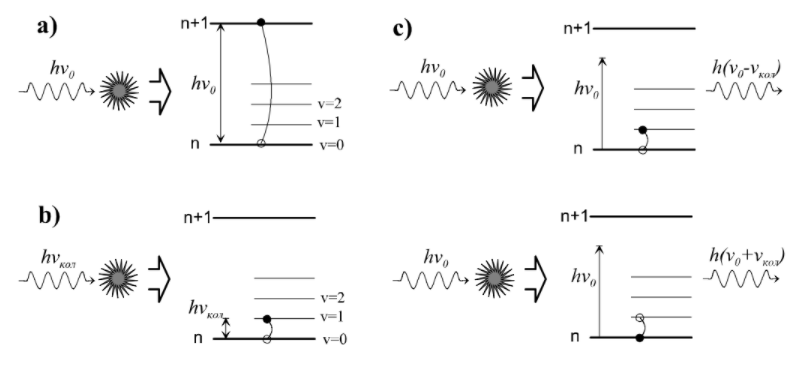
\includegraphics[scale=1]{поглощение-рассеяние.png}
    \caption{Схема процессов при взаимодействии излучения с веществом. a - поглощение в оптической области, b - поглощение в ИК-области, c - кобинационное рассеяние света: сверху - стоксово, снизу - антистоксово}
    \label{Ber}
\end{figure}

Поскольку в основном электронном состоянии молекулы существует
множество колебательных состояний с различными энергиями, то заселенность
этих колебательных состояний подчиняется распределению Больцмана. Выражение для отношения
интенсивностей стоксового и антистоксового рассеянного излучения:
\[\frac{J_s}{J_{a-s}}=\left(\frac{\omega_0 - \omega_1}{\omega_0 + \omega_1}\right)^4\exp{\left[-\frac{h\omega_1}{T}\right]}\]

\subsection{Спектр КРС и колебания молекулы}
Комбинационное рассеяние света связано с изменением поляризуемости
молекул за счет колебаний ядерного скелета молекулы. При этом существенна
именно способность к изменению – производная по нормальной координате, а не величина самой поляризуемости. Произвольное колебание молекулы, содержащей N атомов (у каждого
атома по 3 степени свободы), можно представить как линейную комбинацию
3N-6 базисных колебаний (6 колебаний приводят к вращению или перемещению
молекулы как единого целого). Координаты этих колебаний и сами колебания
называют нормальными или собственными. Нормальные колебания независимы
друг от друга, при каждом нормальном колебании все ядра колеблются с одной
частотой и в фазе.
\begin{figure}[h!]
    \centering
    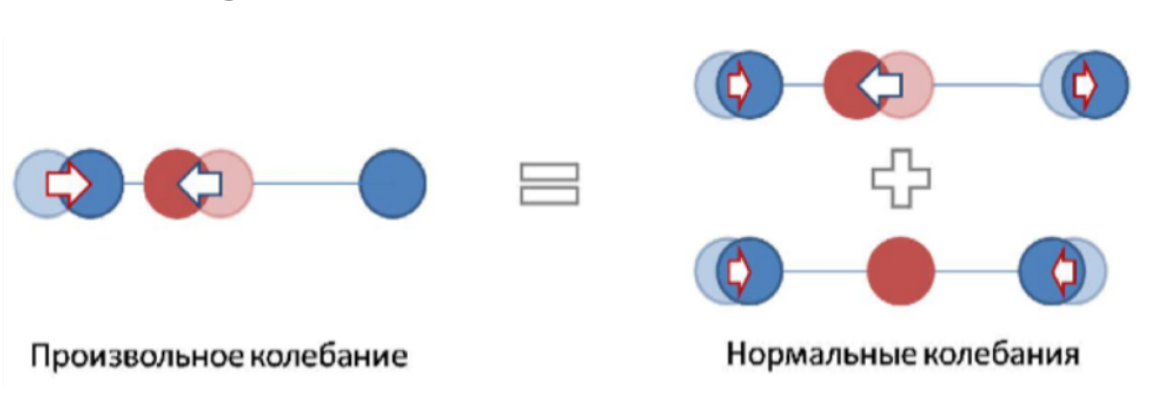
\includegraphics[scale=0.7]{колебания.png}
    \caption{Иллюстрация разложения произвольного колебания на собственные}
    \label{Ber}
\end{figure}

Наиболее простым для рассуждений является случай молекул, обладающих
центром симметрии. В случае симметричных колебаний (относительно центра
симметрии) дипольный момент таких молекул не изменяется. Поляризуемость
молекулы, наоборот, сильно изменяется при таких колебаниях, так как в этом
случае изменяется расстояние между ядрами, а значит, и поле, в котором
находится электронное облако, следовательно, и способность электронного
облака к деформации. В случае антисимметричных колебаний исходная форма
молекулы искажается, что приводит к изменению дипольного момента
молекулы — поляризуемость, однако, при таких колебаниях не меняется
существенно. «правило альтернативного запрета»: в молекулах, обладающих центром симметрии,
нормальное колебание не проявляется в спектрах КРС, если оно проявляется в
ИК-спектрах, и наоборот.

\subsection{Колебания молекул воды и особенности ее спектра КРС}

Молекула воды демонстрирует изгибное деформационное колебание на частоте 1640 ${cm}^{-1}$ (Изгиб может происходить лишь в плоскости самой молекулы.), симметричное и асимметричное растяжение на частотах 3247 и 3450 ${cm}^{-1}$.
Молекула воды не обладает центром симметрии,
поэтому «правило альтернатвного запрета» на нее не распространяется.
Молекула воды обладает дипольным моментом, поэтому все упомянутые выше
колебания приводят к изменению этого самого дипольного момента, и, как
следствие, являются активными в ИК-поглощении.
Изгиб и асимметричное растяжение присутствуют на спектрах КРС, но дают весьма слабые пики (относительно симметричного растяжения). Область волновых чисел ниже 900 ${cm}^{-1}$ соответствует колебаниям молекул целиком вдоль водородных связей и так называемым «крутильным колебаниям» молекул воды, в ходе которых молекулы воды совершают вращательные колебания вокруг водородных связей.

\begin{figure}[h!]
    \centering
    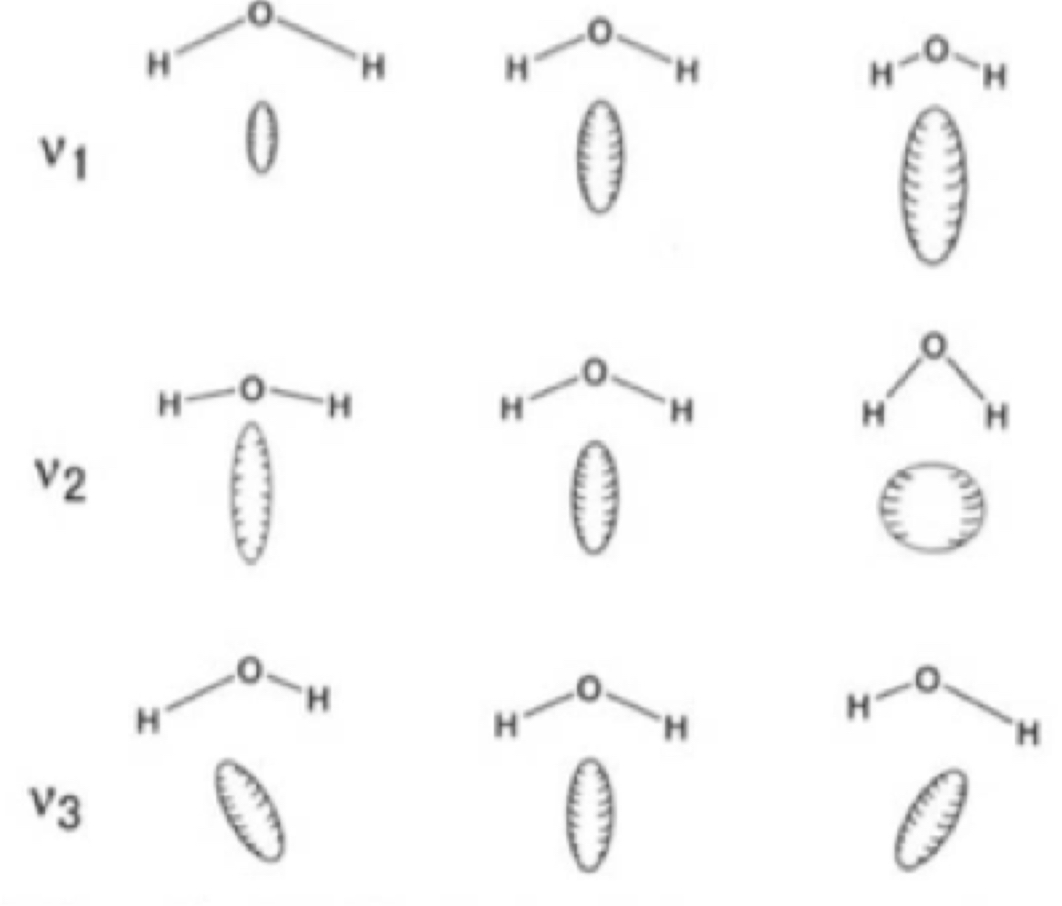
\includegraphics[scale=0.15]{вода.png}
    \caption{Изменение формы эллипсоида
поляризуемости при различных колебаниях
молекулы воды. $\nu_1$ и $\nu_3$ — симметричное и
асимметричное растяжение, $\nu_2$ — деформационный
изгиб.}
    \label{Ber}
\end{figure}

Рассмотрим теперь подробнее область спектра комбинационного рассеяния с волновыми числами 3000-3700 ${cm}^{-1}$. Её в литературе могут называть «валентной полосой» воды. Один из ключевых факторов при интерпретаций сложной формы
рамановской валентной полосы $H_2O$ заключается в том, что разное число молекул воды образует различное число водородных связей (Рис. 5). Эта интерпретация основывается, в частности, на том наблюдении, что повышение температуры вызывает уменьшение интенсивности валентной полосы О-Н в области 3200 ${cm}^{-1}$ и увеличение этой интенсивности в области частот 3600 ${cm}^{-1}$. Эти изменения приписываются большему числу разорванных водородных связей при более высоких температурах.
\begin{figure}[h!]
    \centering
    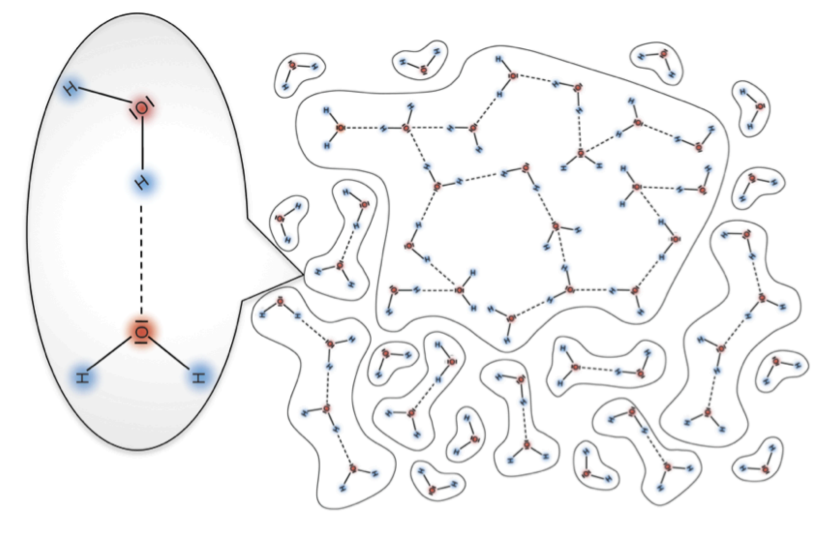
\includegraphics[scale=0.6]{разные водор связи.png}
    \caption{Кластеры молекул воды с различным числом водородных связей.}
    \label{Ber}
\end{figure}

В рамках такого приближения воду можно рассматривать как смесь двух состояний – «полимер», связанный водородными связями и «мономер», состоящий из отдельных молекул воды.

\begin{figure}[h!]
    \centering
    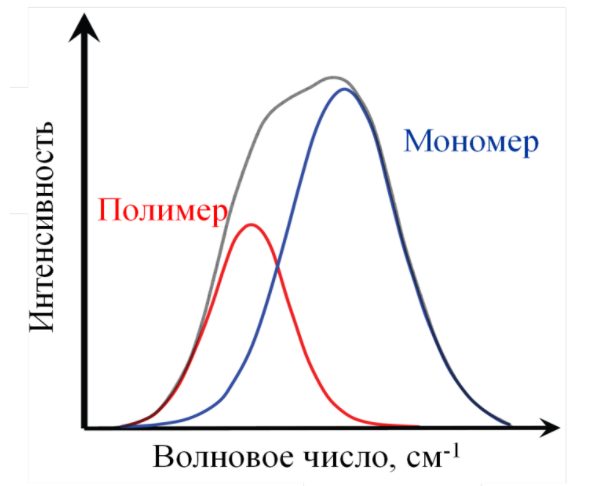
\includegraphics[scale=0.6]{пики.png}
    \caption{Декомпозиция валентной
полосы О-Н на две гауссовые компоненты, соответсвующие мономеру и полимеру.}
    \label{Ber}
\end{figure}

\subsection{Экспериментальная установка}
Схема используемой в работе установки приведена на рисунке ниже. В качестве
источника возбуждающего излучения используется лазерный диод с длиной волны
излучения  445 нм‚ выходная мощность 1 Вт. Лазерное излучение фокусируется в кювету с
исследуемым образцом при помощи линзы. Кювета находится в термостатируемом
кюветодержателе. При помощи термостата осуществляется нагрев и поддержание
заданной при эксперименте температуры. Рассеянное излучение от образца
собирается при помощи второй линзы таким образом, чтобы изображение лазерного луча,
проходящего кювету с образцом, проецировалось на входное отверстие USB-
спектрометра. Перед входным отверстием спектрометра помещается фильтр, отсекающий
излучение с длиной волны короче чем 450 нм (спектр пропускания и оптической
плотности фильтра приведены на рис.1). Это позволяет избавиться от интенсивного
релеевского рассеяния. Спектры регистрируются при помощи программного обеспечения
спектрометра, инструктаж по работе с программой необходимо получить у преподавателя.
Так же в установке может дополнительно использоваться твердотельный лазер с диодной
накачкой, длина волны излучения 532 нм, выходная мощность 0,8 Вт и дополнительный
фильтр, блокирующий 532 нм.
\begin{figure}[h!]
    \centering
    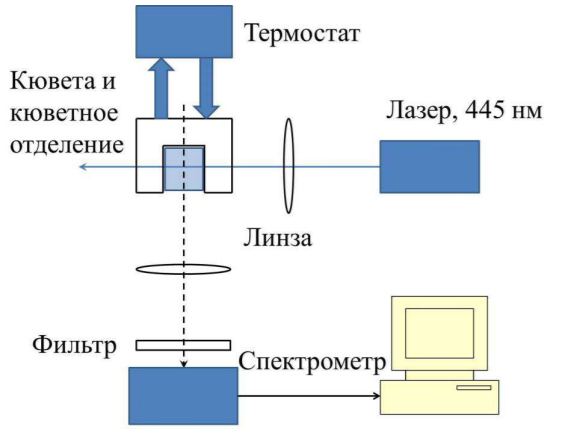
\includegraphics[scale=1]{ustanovka.png}
    \caption{Схема экспериментальной установки}
    \label{Ber}
\end{figure}




\newpage
\section{Ход работы и обработка результатов}
\begin{itemize}
\subsection{Измерение параметров установки}
\subsubsection{Спектр комбинационного рассеяния жидких образцов}
Включим лазер,
установим в кюветное отделение кювету с изопропиловым спиртом. Получим спектр комбинационного рассеяния изопропанола.


Спектры комбинационного рассеяния строятся в координатах (v[см$^{-1}$], I), где волновое число определяется из соотношения
\begin{equation*}
    v = \frac{1}{\lambda_{laser}} - \frac{1}{\lambda}
\end{equation*}


\begin{figure}[h!]
\begin{minipage}[h]{0.49\linewidth}
\center{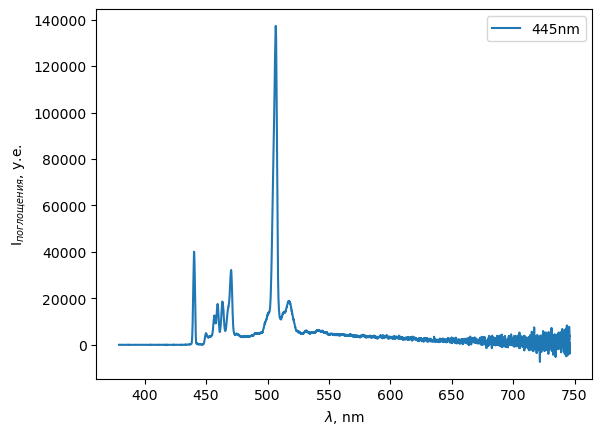
\includegraphics[width=1\linewidth]{isoprop_445.png}} \\
\end{minipage}
\hfill
\begin{minipage}[h]{0.49\linewidth}
\center{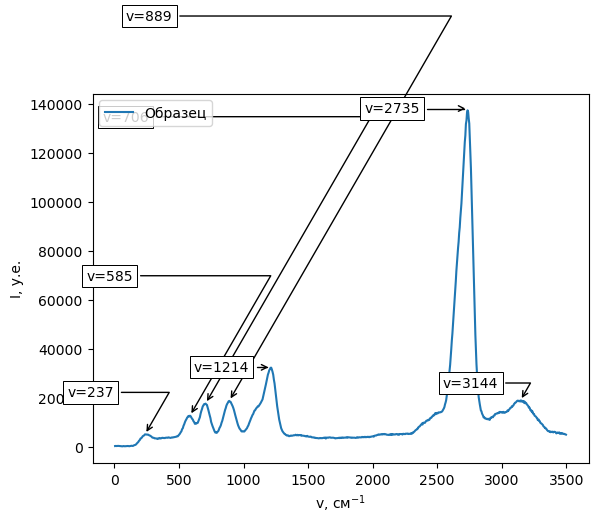
\includegraphics[width=1\linewidth]{spectrum_without_et.png}} \\
\end{minipage}

\caption{\centering Спектр комбинационного рассеяния света изопропанола}

\end{figure} 

\item Погрешность определения пиков находится следующим образом:

 $\sigma \lambda$ = 0.1нм (дискретность измерений установкой)

 $\sigma v = \sigma \lambda / \lambda^2 = \sigma \lambda \left(\frac{1}{\lambda_{laser}}-v\right)^2$

\item Сравним экспериментально опредленные пики с эталонными значениями\\
\begin{table}[h!]
\centering
\begin{tabular}{|l|l|l|l|l|l|l|l|l|l|l|}
\hline
эталон, см$^{-1}$ &
  373 &
  429 &
  489 &
  819 &
  953 &
  1132 &
  1451 &
  2881 &
  2920 &
  2973 \\ \hline
образец,  см$^{-1}$ &
  - &
  - &
  $585 \pm 5 $$&
  $706 \pm 5$ &
  $889 \pm 5$ &
  $1214  \pm 5$ &
  - &
  $2735 \pm 4 $$&
  - &
  - \\ \hline
\end{tabular}
\caption{Сравнение экспериментально определенных пиков спектра КРС изопропанола с эталонными значениями}
\label{tab:my-table}
\end{table}


\item Оценка разрешающией способности установки:\\

Для измерения разрешающей способности установки рассмотрим два соседних пика. Воспользуемся формулой для разрешающей способности:

\begin{equation*}
    R = \frac{\lambda}{\delta \lambda} = \frac{\lambda_1}{\lambda_2 - \lambda_1} = \frac{v_2}{v_2-v_1}, \sigma R = \sqrt{\frac{\sigma^2v_2}{v_2^2} + \frac{\sigma^2v_1+\sigma^2v_2}{(v_2-v_1)^2}}
\end{equation*}

Ближающие разрешенные пики: $v_1=(706\pm5)$см$^{-1}$, $v_2=(889\pm5)$см$^{-1}$
\begin{equation*}
    \boxed{R=4.86\pm 0.04}
\end{equation*}

\item Соответствие пиков спектра КРС со структурой молекулы изопропанола 
\begin{figure}[h!] \label{fig4}
    \centering
    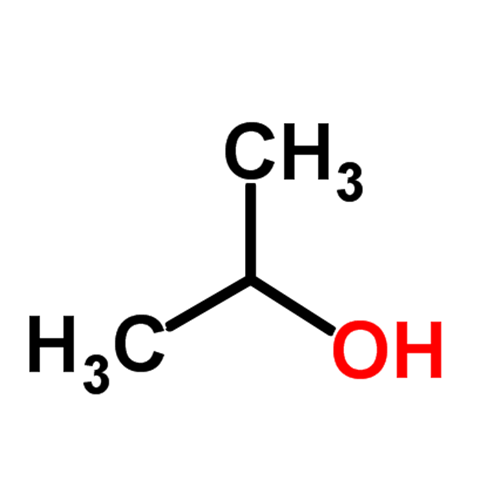
\includegraphics[scale = 0.2]{izopropanol.png}
    \caption{\centering Структурная формула изопропанола}
\end{figure}\\
Можно предположить, что:
\begin{itemize}
    \item 819 см $^{-1}$ - колебания С-С
    \item 953 см $^{-1}$ - колебания С-O
    \item 2881-2973 см $^{-1}$ - колебания СH$_3$, CH и OH
\end{itemize}
\newpage
\subsection{Спектры комбинационного рассеяния воды}
\item Необходимо определить энергию водородных связей в воде. Для этого были сняты спектры комбинационного рассеяния воды при температурах в диапазоне 30-80 С$^\circ$.     

Спектр КРС воды имеет валентную полосу воды - область 3000-3700см$^{-1}$, отвечающая колебаниям водородной связи. В простейшем случае спектр раскладывается на 2 Гауссовы составляющие, одна из которых уменьшается при увеличении температуры (колебания молекул, соединенных водородными связями), а вторая увеличивается (внутримолекулярные валентные моды молекул, не соединённых водородными связями)
связями. У нас не получилось пронаблюдать разделение на 2 Гауссовы составляющие.
\begin{figure}[h!]

\center{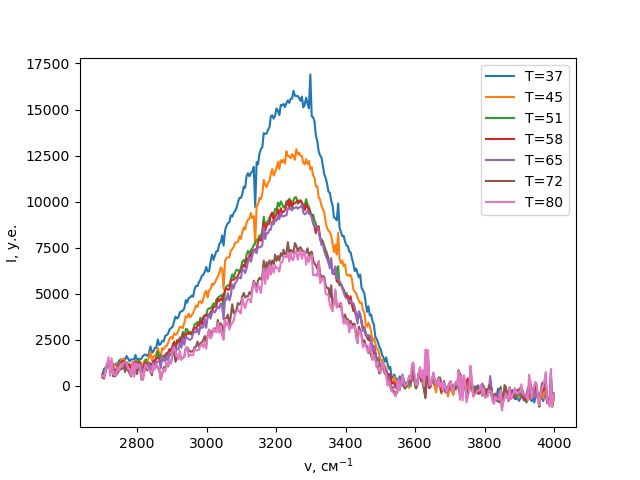
\includegraphics[width=0.7\linewidth]{all.png}} \\
\caption{\centering Изменение валентной полосы воды при увеличении температуры\label{all}
}
\end{figure} 

\item Зависимость энергии водородной связи от формы пика
\begin{itemize}
    \item Переход между мономерным и полимерным состоянием можно описать обратимой реакцией 
\begin{equation*}
    M \leftrightarrow P
\end{equation*}
\item Интенсивность пика пропорциональна числу молекул в данном состоянии, поэтому константа равновесия
\begin{equation*}
    K_c = \frac{[P]}{[M]} = \frac{I_p}{I_m}
\end{equation*}
\item Уравнение Вант-Гоффа: 
\begin{equation*}
    \frac{\partial ln K_c}{\partial T} = \frac{\Delta H}{RT^2}  \Rightarrow lnK_c = -\frac{\Delta H}{RT} + c
\end{equation*}
\item Таким образом, 
\begin{equation*}
    ln\frac{I_p}{I_m} = \frac{-\Delta H}{RT} + c
\end{equation*}\end{itemize}

Таким образом, чтобы определить энергию водородной свзяи $\Delta H$, необходимо найти отношение интенсивности пиков при каждой температуре, построить график зависимости в аррениусовских координатах. В качестве меры интенсивности принимается площадь пиков. 
\item Пики имеют Гауссов вид:
\begin{equation*}
    y = a\cdot e^{-b(x-x_0)^2}
\end{equation*}
Считая, что v, не попавшие в рассматриваемый диапазон, не дают существенного вклада в интеграл, выразим площадь под Гауссовой кривой как 
\begin{equation*}
    I = 2\cdot \int _{x_0}^{+\infty} a\cdot e^{-b(x-x_0)^2}dx = \sqrt{\pi}\frac{a}{\sqrt{b}}
\end{equation*}
\begin{equation*}
    \sigma I = \sqrt{\pi \frac{b^2 \sigma^2a + a^2 \sigma^2b}{b^3}}
\end{equation*}

\begin{table}[h!]
\centering
\begin{tabular}{|l|l|l|l|l|l|l|l|l|}
\hline
T, $^\circC$ &
  1/T \cdot $10^{-6}$, K$^{-1}$ &
  s(1/T) \cdot$10^{-6}$, K$^{-1}$ &
  I_p \cdot $10^{5}$ &
  \begin{tabular}[c]{@{}l@{}}\sigma $I_p$ \\ \cdot $10^{5}$\end{tabular} &
  $I_m$ \cdot $10^{4}$ &
  \sigma $I_m$ \cdot $10^{4}$ &
  $\ln(I_p/I_m)$ &
  \sigma $\ln(I_p/I_m)$ \\ \hline
37 & 3225.8 & 1.0 & 60.1 & 1.3 & 1.8 & 1.2 & 5.1 & 0.3 \\ \hline
45 & 3144.7 & 1.0 & 47.9 & 1.1 & 1.8 & 1.0 & 4.9 & 0.3 \\ \hline
51 & 3086.4 & 1.0 & 38.6 & 0.9 & 1.8 & 0.9 & 4.7 & 0.3 \\ \hline
58 & 3021.1 & 0.9 & 38   & 0.9 & 1.8 & 1.0 & 4.7 & 0.3 \\ \hline
65 & 2958.6 & 0.9 & 36.8 & 0.9 & 1.8 & 0.9 & 4.6 & 0.3 \\ \hline
72 & 2898.6 & 0.8 & 29   & 1.4 & 1.8 & 1.9 & 4.3 & 0.5 \\ \hline
80 & 2832.9 & 0.8 & 27.3 & 1.5 & 1.8 & 1.7 & 4.2 & 0.4 \\ \hline
\end{tabular}
\caption{Интенсивность пиков в зависимости от температуры}
\label{tab:my-table}
\end{table}
По рассчитанным в таблице данным построен график в аррениусовских координатах.
\begin{figure}[h!] 
    \centering
    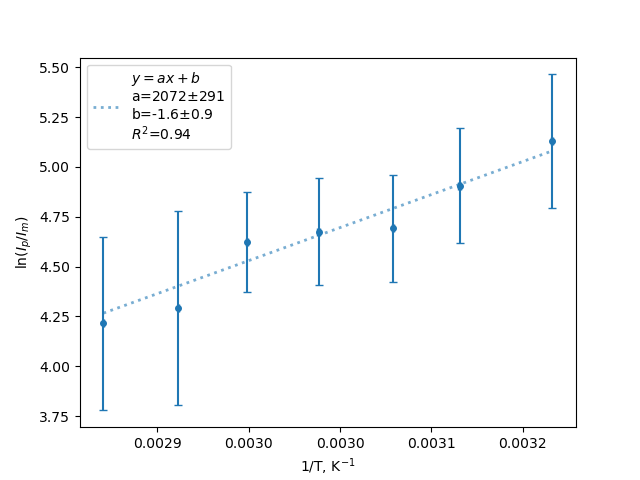
\includegraphics[scale = 0.7]{log_3.png}
    \caption{\centering График зависимости отношения интенсивностей пиков от температуры в аррениусовских координатах \label{fig12}}
\end{figure}


\item Точки графика \ref{fig12} неплохо описываются линейной зависимостью.
\begin{equation*}
    \frac{\Delta H}{R} = -(2072 \pm 291) K^{-1} \Rightarrow\boxed{ \Delta H = -(17.2 \pm 2.4) \text{кДж/моль}}
\end{equation*}

\end{itemize}










\section{Вывод}
 В ходе работы были исследованы спектры комбинационного рассеяния изопропанола и воды. 

\begin{itemize}
    \item По спектру изопропанола была оценена разрешающая способность установки $R = 4.86 \pm 0.04$. 


 \item По спектру комбинационного рассеяния воды была рассчитана энергия водородной связи в воде $E_{H-bond}=(17.2\pm2.4)$ кДж/моль. Табличное значение $E = 21.5$ кДж/моль. Не получилось пронаблюдать разделение зависимости на 2 Гауссовы составляющие.
 \end{itemize}

\newpage

\section{Приложение}
\begin{figure}[h!]
\begin{minipage}[h!]{0.49\linewidth}
\center{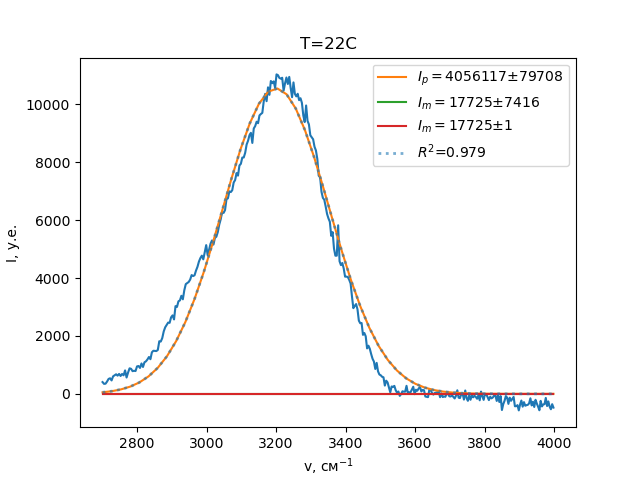
\includegraphics[width=1\linewidth]{22_3.png}} \\
\end{minipage}
\hfill
\begin{minipage}[h!]{0.49\linewidth}
\center{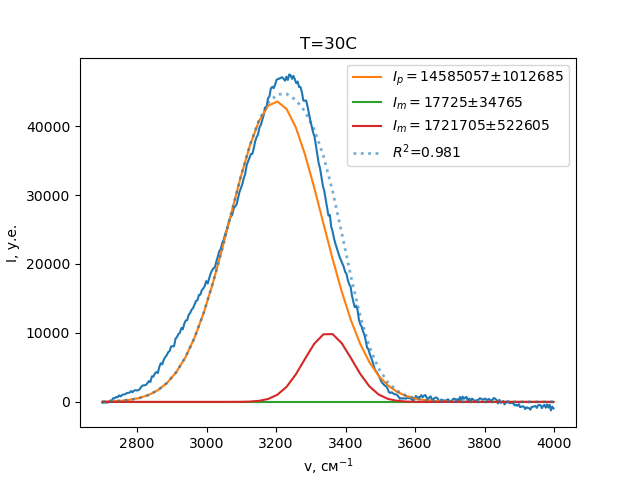
\includegraphics[width=1\linewidth]{30_3.png}} \\
\end{minipage}
\end{figure} 
\begin{figure}[h!]
\begin{minipage}[h]{0.49\linewidth}
\center{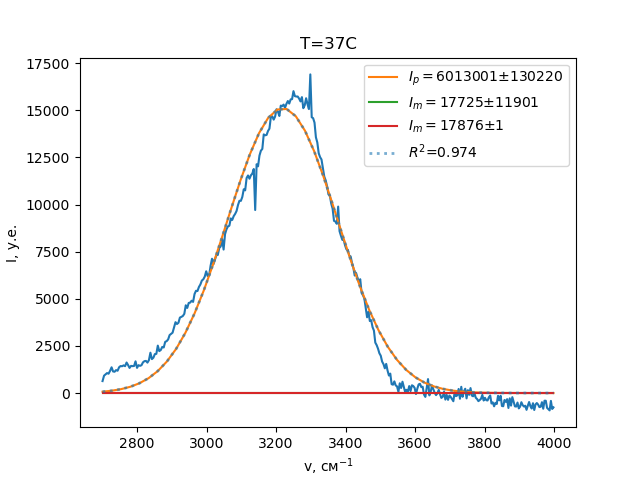
\includegraphics[width=1\linewidth]{37_3.png}} \\
\end{minipage}
\hfill
\begin{minipage}[h!]{0.49\linewidth}
\center{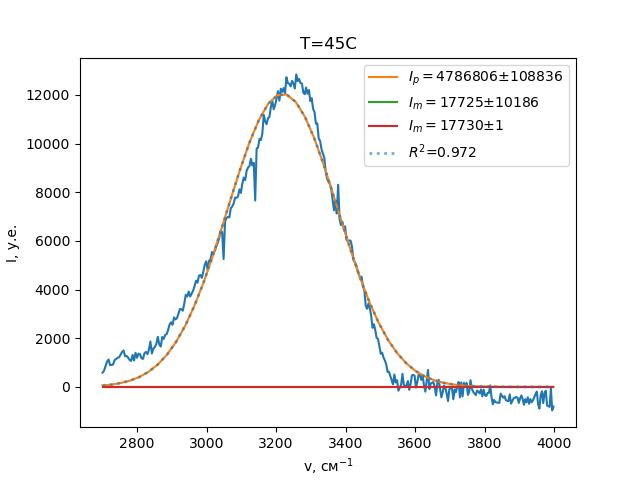
\includegraphics[width=1\linewidth]{45_3.png}} \\
\end{minipage}
\end{figure} 
\begin{figure}[h!]
\begin{minipage}[h]{0.49\linewidth}
\center{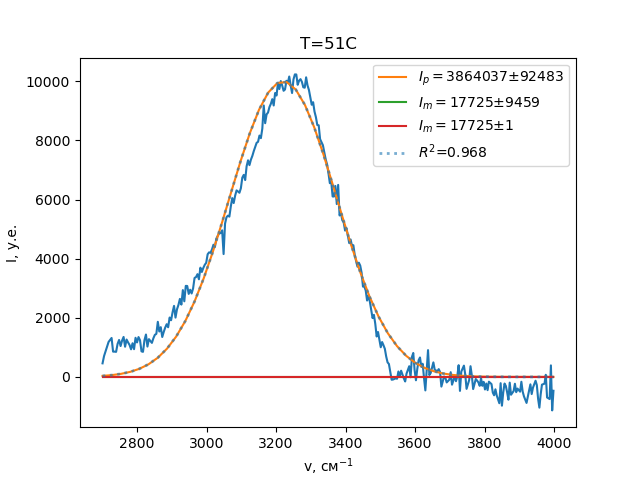
\includegraphics[width=1\linewidth]{51_3.png}} \\
\end{minipage}
\hfill
\begin{minipage}[h!]{0.49\linewidth}
\center{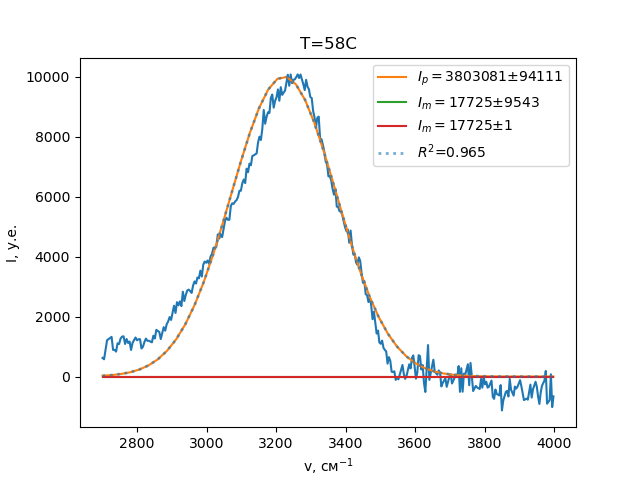
\includegraphics[width=1\linewidth]{58_3.png}} \\
\end{minipage}
\end{figure} 


\begin{figure}[h!]
\begin{minipage}[h]{0.49\linewidth}
\center{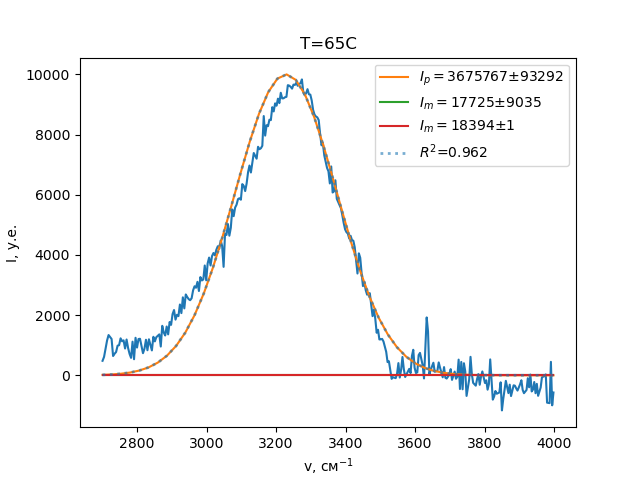
\includegraphics[width=1\linewidth]{65_3.png}} \\
\end{minipage}
\hfill
\begin{minipage}[h]{0.49\linewidth}
\center{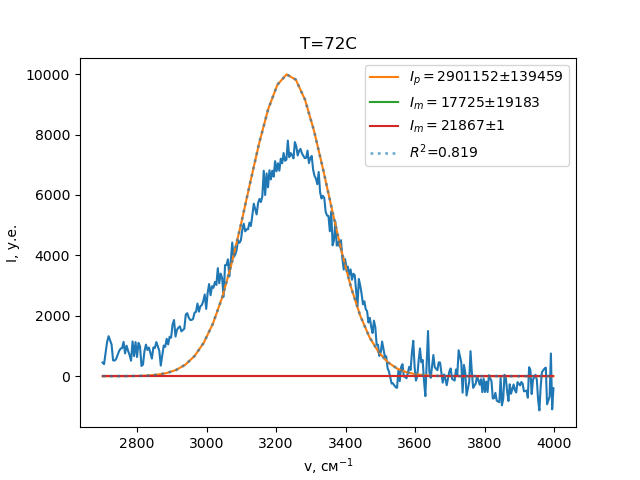
\includegraphics[width=1\linewidth]{72_3.png}} \\
\end{minipage}
\end{figure} 

\begin{figure}[h!]
\begin{minipage}[h]{0.49\linewidth}
\center{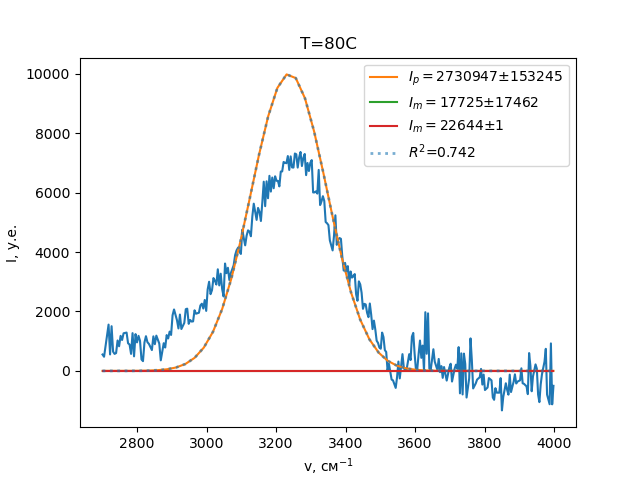
\includegraphics[width=1\linewidth]{80_3.png}} \\
\end{minipage}

\end{figure} 

\end{document}